\documentclass[xcolor={dvipsnames,rgb}]{beamer}

\beamertemplatenavigationsymbolsempty

\usepackage{tikz}
\usepackage{amsmath}
\usepackage{amssymb}
\usepackage{mathtools}

\usetikzlibrary{positioning}
\usetikzlibrary{backgrounds}
\usetikzlibrary{tikzmark}
\usetikzlibrary{shapes,arrows,calc}

\newcommand{\highlight}[2]{\colorbox{#1}{$\mathstrut #2$}}

\definecolor{variable}{HTML}{999999}
\definecolor{operator}{HTML}{bbbbbb}
\definecolor{vtrue}{HTML}{66ff66}
\definecolor{vfalse}{HTML}{ff6666}
\definecolor{rtrue}{HTML}{aaffaa}
\definecolor{rfalse}{HTML}{ffaaaa}

\tikzstyle{into} = [draw, -triangle 45, shorten >=0pt]

\tikzstyle{label} = [minimum height=2em, minimum width=2em]
\tikzstyle{var} = [draw, rectangle, minimum height=2em, minimum width=2em, fill=variable]
\tikzstyle{oper} = [draw, rectangle, minimum height=2em, minimum width=2em, fill=operator]
\tikzstyle{it} = [draw, diamond, minimum height=2em, minimum width=2em, fill=vtrue]
\tikzstyle{if} = [draw, circle, minimum height=2em, minimum width=2em, fill=vfalse]
\tikzstyle{ot} = [draw, diamond, minimum height=2em, minimum width=2em, fill=rtrue]
\tikzstyle{of} = [draw, circle, minimum height=2em, minimum width=2em, fill=rfalse]



% https://i.stack.imgur.com/2X1Jv.png
\colorlet{ca}{Peach!30}
\colorlet{co}{Goldenrod!30}
\colorlet{cn}{Tan}
\colorlet{ci}{Sepia!30}


\begin{document}

\begin{frame}{\textit{Truth table} for the \textbf{binary} operator $\leftrightarrow$}

  \begin{center}
    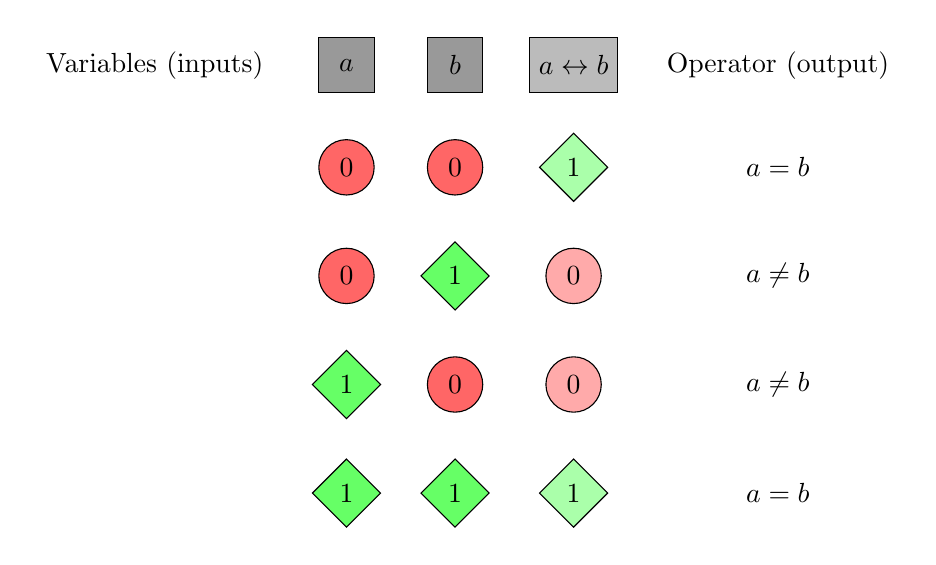
\begin{tikzpicture}[ampersand replacement=\&]
      \matrix[row sep = 5mm, column sep = 5mm] at (0, 0) {
        \onslide<2->{ \node[label]{Variables (inputs)}; }
        \& \node[var]{$a$}; 
        \& \node[var]{$b$};
        \& \node[oper]{$a \leftrightarrow b$};
        \& \onslide<2->{ \node[label]{Operator (output)}; }
        \\
        \& \onslide<3-18,22->{ \node[if]{0}; }
        \&  \onslide<4-18,22->{ \node[if]{0}; }
        \&  \onslide<5-18,22->{ \node[ot]{1}; }
        \&  \onslide<16-18,22->{ \node[label]{$a = b$}; }
        \\
        \&  \onslide<6-15,19->{ \node[if]{0}; }
        \&  \onslide<7-15,19->{ \node[it]{1}; }
        \&  \onslide<8-15,19->{ \node[of]{0}; }
        \&  \onslide<19-21,19->{ \node[label]{$a \neq b$}; }
        \\
        \& \onslide<9-15,19->{ \node[it]{1}; }
        \&  \onslide<10-15,19->{ \node[if]{0}; }
        \&  \onslide<11-15,19->{ \node[of]{0}; }
        \&  \onslide<19-21,19->{ \node[label]{$a \neq b$}; }
        \\
        \&  \onslide<12-18,22->{ \node[it]{1}; }
        \&  \onslide<13-18,22->{ \node[it]{1}; }
        \&  \onslide<14-18,22->{ \node[ot]{1}; }
        \&  \onslide<16-18,22->{ \node[label]{$a = b$}; }
        \\        
      }; 
    \end{tikzpicture}

  
  \onslide<22->{ This is called \textit{equivalence}. }
  
  \onslide<23-27>{ Note that $a \leftrightarrow b$ is the same as $\neg (a \oplus b)$. }

    
  \end{center}


  
\end{frame}

\end{document}
